\begin{subfigure}{0.32\columnwidth}
        \vspace{1.05cm}
        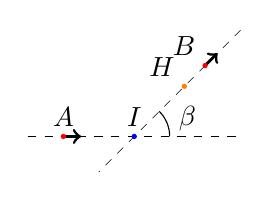
\begin{tikzpicture}[scale=0.45]
            \coordinate[label=above:$A$] (A) at (0,0);
            \coordinate[label=135:$B$] (B) at (4,2);
            \coordinate[label=above:$I$] (iP) at (2,0);
            \coordinate[label=135:$H$] (H) at (3.41421,1.41421);
        
            \draw[dashed, line width=0.2] (-1,0) -- (5,0);
            \draw[dashed, line width=0.2] (5,3) -- (1,-1);
            \draw (3,0) arc (0:45:1);
        
            \draw[->, line width=1] (A) -- (0.5,0);
            \draw[->, line width=1] (B) -- (4.35,2.35);
            \fill[red] (A) circle (0.075);
            \fill[red] (B) circle (0.075);
            \fill[blue] (iP) circle (0.075);
            \fill[orange] (H) circle (0.075);
        
            \draw (3.5, 0.5) node {$\beta$};
        \end{tikzpicture}
        \caption{find helping point}
        \label{fig_construct_hp}
        \end{subfigure}
        \begin{subfigure}{0.32\columnwidth}
            \begin{tikzpicture}[scale=0.45]
                \coordinate[label=below:$A$] (A) at (0,0);
                \coordinate[label=135:$B$] (B) at (4,2);
                \coordinate[] (iP) at (2,0);
                \coordinate[] (H) at (3.41421,1.41421);
                \coordinate[] (E) at (0,4.8284);
                \coordinate[] (F) at ($(A)!0.5!(H)$);
            
                \draw[dashed, line width=0.2] (-1,0) -- (5,0);
                \draw[dashed, line width=0.2] (5,3) -- (1,-1);
            
                \draw[blue, line width = 1] (H) -- (B);
            
                \draw[->, black, line width=1] (A) -- (0.5,0);
                \draw[->, black, line width=1] (H) -- (3.7676,1.7676);
            
                \draw[label=below:$d$] (A) -- (H);
                \draw[line width=1] (A) arc (-90:-45:4.8284);
                \draw (0,4.3284) arc (-90:-45:0.5);
                \draw[dashed] (A) -- (E) -- (H);
                \draw[] (E) -- (F);
            
                \fill[red] (A) circle (0.075);
                \fill[red] (B) circle (0.075);
                \fill[blue] (iP) circle (0.075);
                \fill[orange] (H) circle (0.075);
                \fill[black] (E) circle (0.05);
            
                \draw (-0.35,2)  node {r};
                \draw (2.4,1.4) node {d};
                \draw (0.25,4.5) -- (0.6,4.7);
                \draw (0.75, 4.7) node {$\frac{\beta}{2}$};
            
            \end{tikzpicture}
        \caption{arc construction}
        \end{subfigure}
        \begin{subfigure}{0.32\columnwidth}
            \vspace{1cm}
        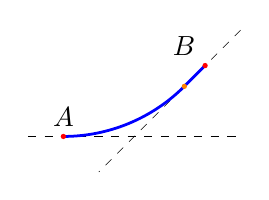
\begin{tikzpicture}[scale=0.45]
            
            \coordinate[label=above:$A$] (A) at (0,0);
            \coordinate[label=135:$B$] (B) at (4,2);
            \coordinate[] (H) at (3.41421,1.41421);
        
            \draw[dashed, line width=0.2] (-1,0) -- (5,0);
            \draw[dashed, line width=0.2] (5,3) -- (1,-1);
        
            \draw[blue, line width=1] (H) -- (B);
            \draw[blue, line width=1] (A) arc (-90:-45:4.8284);
        
            \fill[red] (A) circle (0.075);
            \fill[red] (B) circle (0.075);
            \fill[orange] (H) circle (0.075);
        
        \end{tikzpicture}
        \caption{connected road}
        \end{subfigure}